\documentclass[tikz,border=2pt]{standalone}

\usepackage{tikz}
\usepackage{amsfonts}

\begin{document}

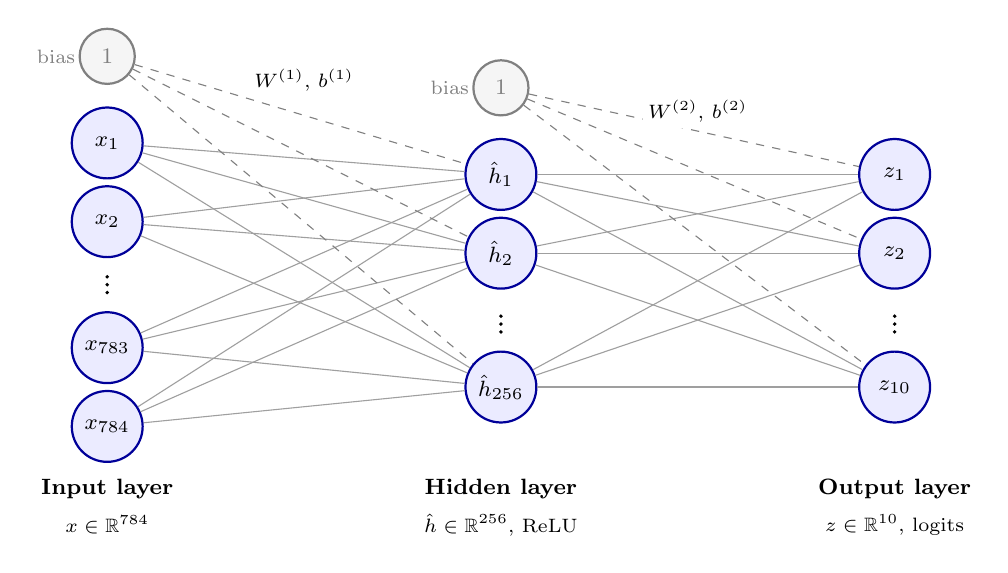
\begin{tikzpicture}[
    font=\footnotesize,
    neuron/.style={circle, draw=blue!60!black, thick, fill=blue!8,
                   minimum size=9mm, inner sep=0pt},
    bias/.style={circle, draw=gray, thick, fill=gray!8, text=gray,
                 minimum size=7mm, inner sep=0pt},
    conn/.style={draw=gray!75, thin},
    biasconn/.style={draw=gray, thin, dashed},
    layerlabel/.style={align=center, font=\footnotesize\bfseries},
    tensorlabel/.style={align=center, font=\scriptsize}
]
    \node[neuron] (i1) at (0,2.2) {$x_1$};
    \node[neuron] (i2) at (0,1.2) {$x_2$};
    \foreach \y in {0.50,0.40,0.30}
        \fill (0,\y) circle (0.7pt);
    \node[neuron] (i783) at (0,-0.4) {$x_{783}$};
    \node[neuron] (i784) at (0,-1.4) {$x_{784}$};
    \node[bias] (ibias) at (0,3.3) {$1$};

    \node[neuron] (h1) at (5,1.8) {$\hat{h}_1$};
    \node[neuron] (h2) at (5,0.8) {$\hat{h}_2$};
    \foreach \y in {0.0,-0.1,-0.2}
        \fill (5,\y) circle (0.7pt);
    \node[neuron] (h256) at (5,-0.9) {$\hat{h}_{256}$};
    \node[bias] (hbias) at (5,2.9) {$1$};

    \node[neuron] (z1) at (10,1.8) {$z_1$};
    \node[neuron] (z2) at (10,0.8) {$z_2$};
    \foreach \y in {0.0,-0.1,-0.2}
        \fill (10,\y) circle (0.7pt);
    \node[neuron] (z10) at (10,-0.9) {$z_{10}$};

    \foreach \i in {i1,i2,i783,i784}
        \foreach \h in {h1,h2,h256}
            \draw[conn] (\i) -- (\h);

    \foreach \h in {h1,h2,h256}
        \foreach \z in {z1,z2,z10}
            \draw[conn] (\h) -- (\z);

    \foreach \h in {h1,h2,h256}
        \draw[biasconn] (ibias) -- (\h);

    \foreach \z in {z1,z2,z10}
        \draw[biasconn] (hbias) -- (\z);

    \node[layerlabel] at (0,-2.2) {Input layer};
    \node[tensorlabel] at (0,-2.65) {$x \in \mathbb{R}^{784}$};

    \node[layerlabel] at (5,-2.2) {Hidden layer};
    \node[tensorlabel] at (5,-2.65) {$\hat{h} \in \mathbb{R}^{256}$, ReLU};

    \node[layerlabel] at (10,-2.2) {Output layer};
    \node[tensorlabel] at (10,-2.65) {$z \in \mathbb{R}^{10}$, logits};

    \node[font=\scriptsize, fill=white, inner sep=2pt] at (2.5,3.0)
        {$W^{(1)},\,b^{(1)}$};
    \node[font=\scriptsize, fill=white, inner sep=2pt] at (7.5,2.6)
        {$W^{(2)},\,b^{(2)}$};

    \node[font=\scriptsize, text=gray] at (-0.65,3.3) {bias};
    \node[font=\scriptsize, text=gray] at (4.35,2.9) {bias};

\end{tikzpicture}

\end{document}
